\documentclass{article}

\usepackage{geometry}
\geometry{left=1.5in,right=1.5in,top=1.25in,bottom=1.25in}
\usepackage{listings}
\usepackage{color}
\usepackage{xcolor}
\usepackage{graphicx}
\graphicspath{ {img/} }
\usepackage[bahasa]{babel}

\definecolor{codegreen}{rgb}{0,0.6,0}
\definecolor{codeblue}{rgb}{0,0,0.6}
\definecolor{codegray}{rgb}{0.5,0.5,0.5}
\definecolor{codepurple}{rgb}{0.58,0,0.82}
\definecolor{backcolour}{rgb}{0.95,0.95,0.92}

\lstdefinestyle{mystyle}{
    backgroundcolor=\color{backcolour},   
    commentstyle=\color{codegray},
    keywordstyle=\color{codepurple}\bfseries,
    numberstyle=\tiny\color{codegray}\ttfamily,
    stringstyle=\color{codegreen},
    identifierstyle=\color{codeblue},
    basicstyle=\scriptsize\ttfamily, xleftmargin=2em,frame=single,framexleftmargin=1.5em,  
	rulecolor=\color{codegray},
    breaklines=true,                  
    keepspaces=true,               
    captionpos=b,                  
    numbers=left,                    
    numbersep=5pt,                  
    showspaces=false,                
    showstringspaces=false,
    showtabs=false,                  
    tabsize=2,
    language=Python,
    morecomment=[s]{"""}{"""},
}
 
\lstset{style=mystyle}
 
\title{Tugas Kecil Penyelesaian Persoalan TSP dengan Algoritma \textit{Branch and Bound}}
\author{Dery Rahman A, 13515097, K-01}
\date{Rabu, 5 April 2017}

\begin{document}

	\pagenumbering{gobble}
	\maketitle

	\newpage
	\pagenumbering{arabic}

	\section{Deskripsi Permasalahan}
	\par \textit{Travel Salesman Problem} (TSP) merupakan permasalahan dimana seorang salesman harus mengunjungi semua kota. Dan pada setiap kota tersebut salesman harus mengunjungi sekali kemudian kembali ke kota asal. Tujuannya adalah menentukan rute degan jarak total paling minimum.
	\par Salah satu penyelesaian TSP dapat menggunakan Algoritma \textit{Branch and Bound}. Nilai \textit{bound} yang dihitung dengan menggunakan \textit{reduced cost matrix} dan Bobot Tur Lengkap. Untuk penyelesaian dengan memanfaatkan reduced cost matrix, digunakan matriks yang merepresentasikan graf berarah. Sedangkan untuk penyelesaian dengan Bobot Tur Lengkap, masukan berupa matriks yang merepresentasikan graf tidak berarah.
	\par Masukan: file external dengan matriks yang merepresentasikan bobot dari graf
	
	\par Keluaran:
\begin{enumerate}
	\setlength\itemsep{0em}
	\item Tur terpendek dan bobotnya
    \item Waktu eksekusi    
    \item Jumlah simpul yang dibangkitkan
    \item Gambar graf
    \item Gambar tur terpendek (dinyatakan sebagai warna yang berbeda di dalam graf)
\end{enumerate}

	\section{Kode program}
	
	\lstinputlisting[language=Python,caption=Implementasi \textit{Branch and Bound} dengan \textit{Reduction Cost Matrix}]{../src/reduction_cost.py}
	\lstinputlisting[language=Python,caption=Implementasi \textit{Branch and Bound} dengan Bobot Tur Lengkap]{../src/complete_tour.py}
	\lstinputlisting[language=Python,caption=Implementasi fungsi untuk menggambar \textit{Graph}]{../src/graph.py}

	\section{\textit{Screenshoot Output}}
	
	\begin{figure}[htbp]
 	\centering
  	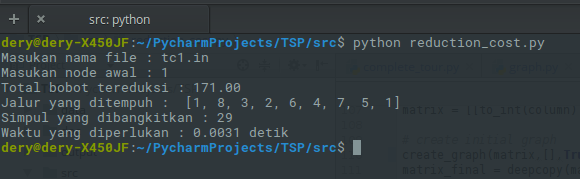
\includegraphics[width=10.5cm, height=3cm]{rcm_1.png}
  	\caption{Hasil \textit{test case 1} dari RCM}
	\end{figure}
	\begin{figure}[htbp]
	\centering
  	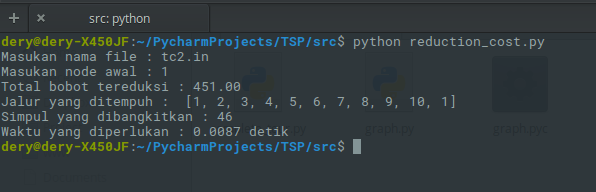
\includegraphics[width=10.5cm, height=3cm]{rcm_2.png}
  	\caption{Hasil \textit{test case 2} dari RCM}
  	\vspace{5mm}
  	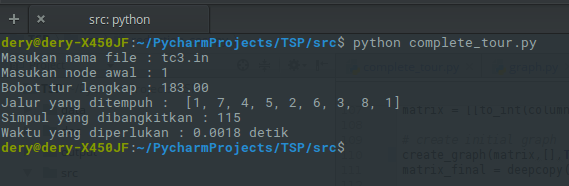
\includegraphics[width=10.5cm, height=3cm]{com_1.png}
  	\caption{Hasil \textit{test case 1} dari Bobot Tur Lengkap}
  	\vspace{5mm}
  	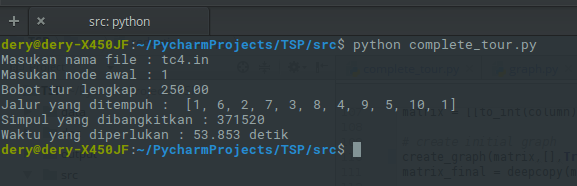
\includegraphics[width=10.5cm, height=3cm]{com_2.png}
  	\caption{Hasil \textit{test case 2} dari Bobot Tur Lengkap}
	\end{figure}
	
	\begin{figure}[htbp]
 	\centering
	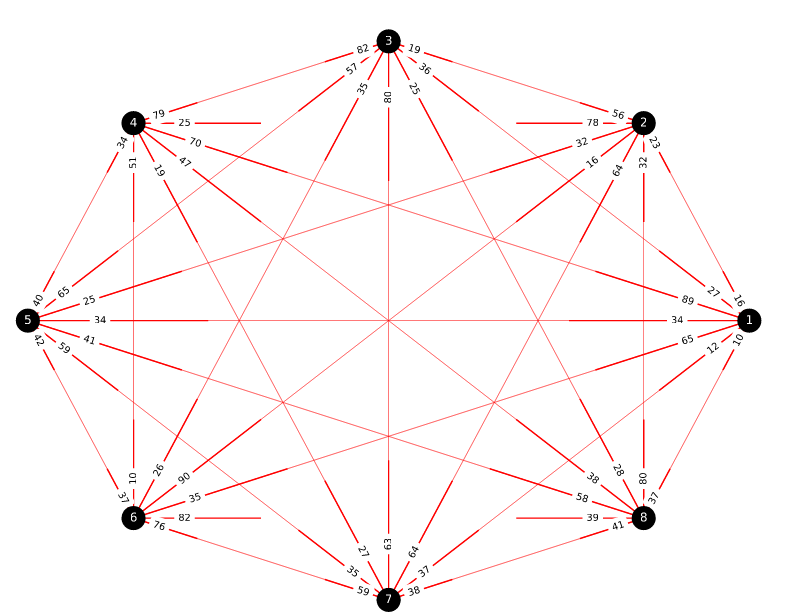
\includegraphics[width=8cm, height=6.5cm]{tc1_i.png}
	\caption{Graf \textit{test case 1}}
	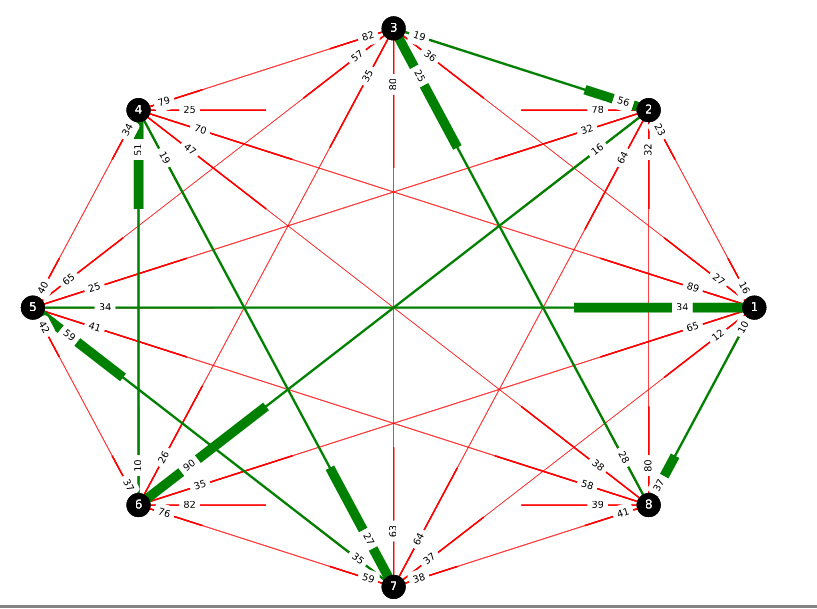
\includegraphics[width=8cm, height=6.5cm]{tc1.png}
	\caption{Graf hasil \textit{test case 1} dari RCM}
	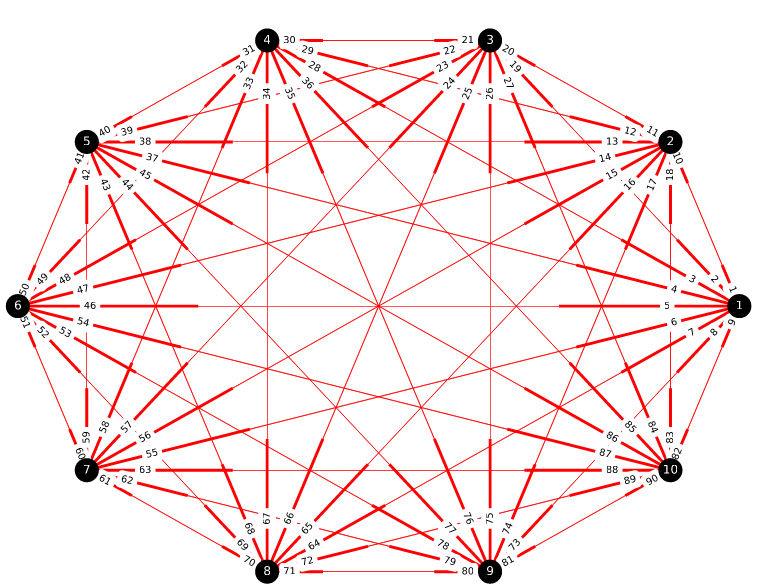
\includegraphics[width=8cm, height=6.5cm]{tc2_i.png}
	\caption{Graf \textit{test case 2}}
	\end{figure}
	
	\begin{figure}[htbp]
	\centering
	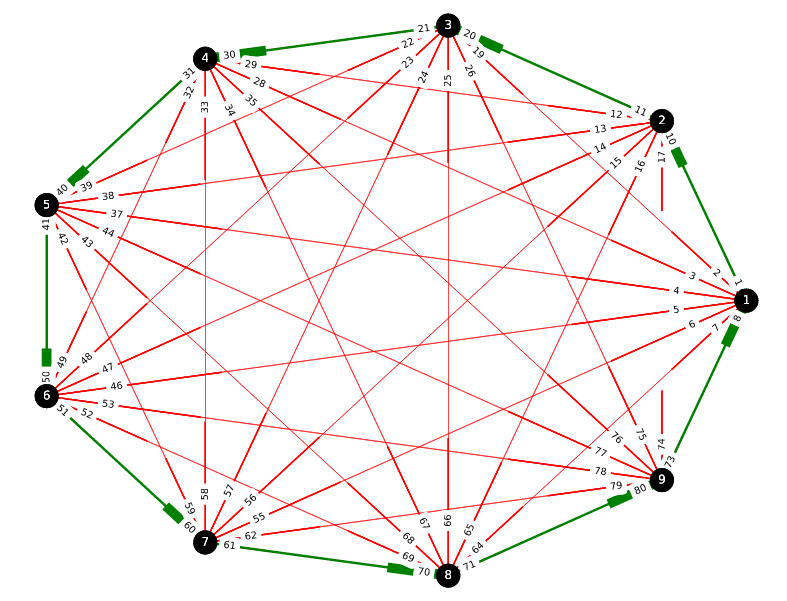
\includegraphics[width=8cm, height=6.5cm]{tc2.png}
	\caption{Graf hasil \textit{test case 2} dari RCM}
	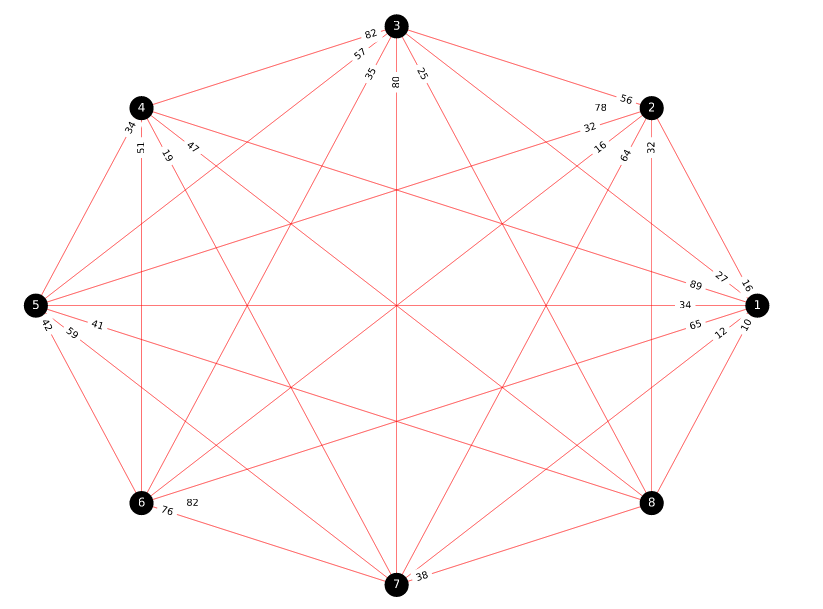
\includegraphics[width=8cm, height=6.5cm]{tc3_i.png}
	\caption{Graf \textit{test case 1}}
	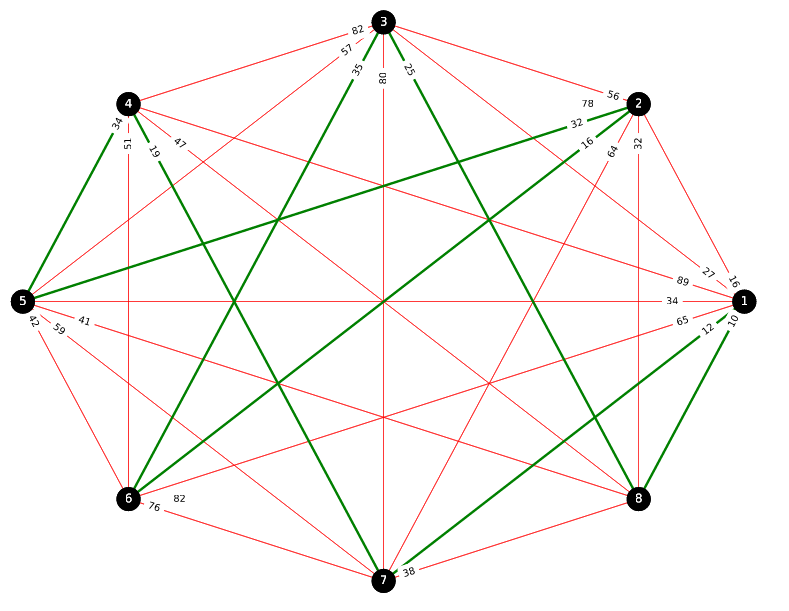
\includegraphics[width=8cm, height=6.5cm]{tc3.png}
	\caption{Graf hasil \textit{test case 1} dari Bobot Tur Lengkap}
	\end{figure}
	
	\begin{figure}[htbp]
	\centering
	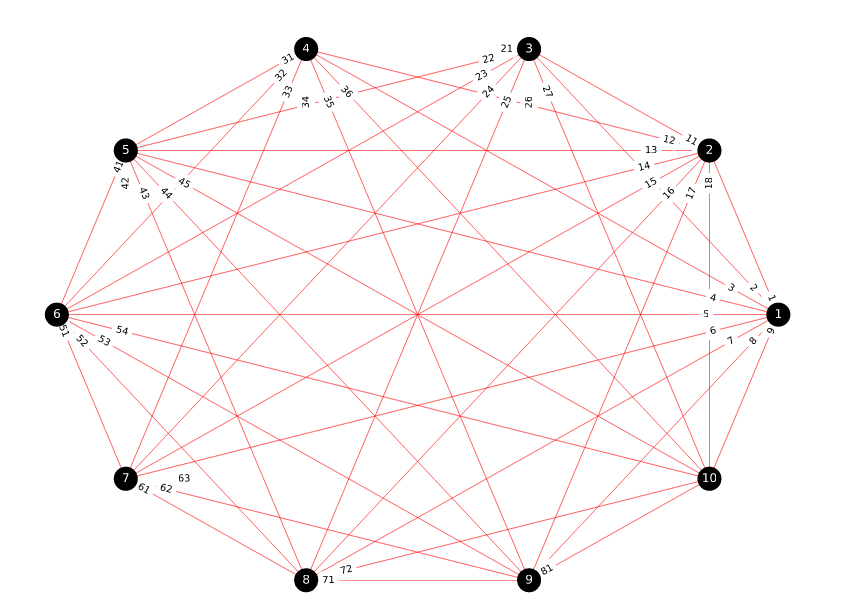
\includegraphics[width=8cm, height=6.5cm]{tc4_i.png}
	\caption{Graf \textit{test case 2}}
	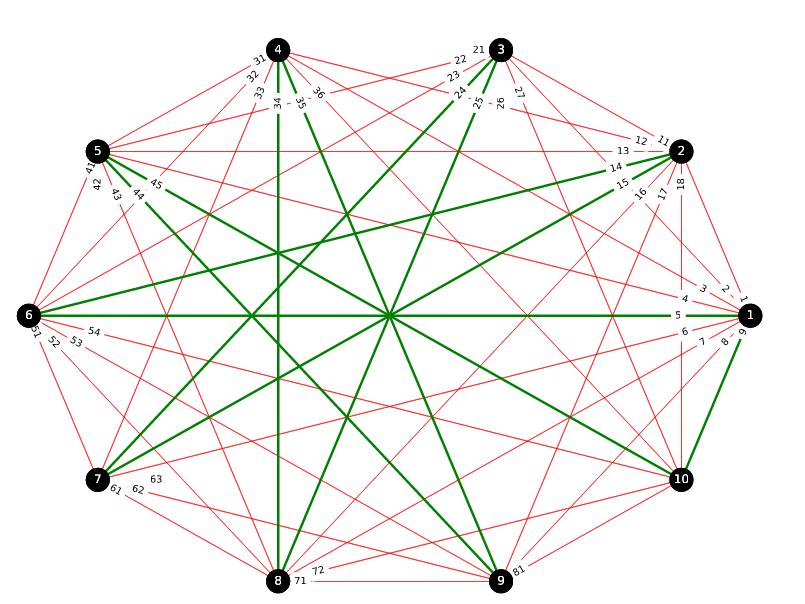
\includegraphics[width=8cm, height=6.5cm]{tc4.png}
	\caption{Graf hasil \textit{test case 2} dari Bobot Tur Lengkap}
	\end{figure}
	
\end{document}
